\documentclass[12pt,]{article}
\usepackage{lmodern}
\usepackage{amssymb,amsmath}
\usepackage{ifxetex,ifluatex}
\usepackage{fixltx2e} % provides \textsubscript
\ifnum 0\ifxetex 1\fi\ifluatex 1\fi=0 % if pdftex
  \usepackage[T1]{fontenc}
  \usepackage[utf8]{inputenc}
\else % if luatex or xelatex
  \ifxetex
    \usepackage{mathspec}
  \else
    \usepackage{fontspec}
  \fi
  \defaultfontfeatures{Ligatures=TeX,Scale=MatchLowercase}
    \setmainfont[]{Calibri Light}
\fi
% use upquote if available, for straight quotes in verbatim environments
\IfFileExists{upquote.sty}{\usepackage{upquote}}{}
% use microtype if available
\IfFileExists{microtype.sty}{%
\usepackage{microtype}
\UseMicrotypeSet[protrusion]{basicmath} % disable protrusion for tt fonts
}{}
\usepackage[left=1in,right=1in,top=1in,bottom=1in]{geometry}
\usepackage{hyperref}
\hypersetup{unicode=true,
            pdftitle={Combinging Multiple Imputation and Cross-Validation for Predicting Survival of ECMO Treatment in ARDS Patients},
            pdfborder={0 0 0},
            breaklinks=true}
\urlstyle{same}  % don't use monospace font for urls
\usepackage{natbib}
\bibliographystyle{plainnat}
\usepackage{longtable,booktabs}
\usepackage{graphicx,grffile}
\makeatletter
\def\maxwidth{\ifdim\Gin@nat@width>\linewidth\linewidth\else\Gin@nat@width\fi}
\def\maxheight{\ifdim\Gin@nat@height>\textheight\textheight\else\Gin@nat@height\fi}
\makeatother
% Scale images if necessary, so that they will not overflow the page
% margins by default, and it is still possible to overwrite the defaults
% using explicit options in \includegraphics[width, height, ...]{}
\setkeys{Gin}{width=\maxwidth,height=\maxheight,keepaspectratio}
\IfFileExists{parskip.sty}{%
\usepackage{parskip}
}{% else
\setlength{\parindent}{0pt}
\setlength{\parskip}{6pt plus 2pt minus 1pt}
}
\setlength{\emergencystretch}{3em}  % prevent overfull lines
\providecommand{\tightlist}{%
  \setlength{\itemsep}{0pt}\setlength{\parskip}{0pt}}
\setcounter{secnumdepth}{5}
% Redefines (sub)paragraphs to behave more like sections
\ifx\paragraph\undefined\else
\let\oldparagraph\paragraph
\renewcommand{\paragraph}[1]{\oldparagraph{#1}\mbox{}}
\fi
\ifx\subparagraph\undefined\else
\let\oldsubparagraph\subparagraph
\renewcommand{\subparagraph}[1]{\oldsubparagraph{#1}\mbox{}}
\fi

%%% Use protect on footnotes to avoid problems with footnotes in titles
\let\rmarkdownfootnote\footnote%
\def\footnote{\protect\rmarkdownfootnote}

%%% Change title format to be more compact
\usepackage{titling}

% Create subtitle command for use in maketitle
\providecommand{\subtitle}[1]{
  \posttitle{
    \begin{center}\large#1\end{center}
    }
}

\setlength{\droptitle}{-2em}

  \title{Combinging Multiple Imputation and Cross-Validation for Predicting
Survival of ECMO Treatment in ARDS Patients}
    \pretitle{\vspace{\droptitle}\centering\huge}
  \posttitle{\par}
    \author{}
    \preauthor{}\postauthor{}
    \date{}
    \predate{}\postdate{}
  
\usepackage[bottom]{footmisc} \usepackage{float}
\floatplacement{figure}{H} \usepackage{color} \usepackage[table]{xcolor}
\usepackage{multirow} \usepackage{caption}
\captionsetup[table]{skip=5pt, font=footnotesize}
\usepackage[font=footnotesize]{caption} \usepackage{algorithm2e}
\usepackage{amsmath}

\begin{document}
\maketitle

\vspace{4cm}

\begin{center}
Robert Edwards 

\vspace{0.125cm}
2416963E


\vspace{1cm}
MASTERS THESIS 

\vspace{0.125cm}
Biostatistics

\vspace{9cm}
  
\includegraphics[height = 1.5cm]{images/GUlogo.png}
\end{center}

\newpage

\begin{center}
~
 
\vspace{5cm}
Acknowledgements 

\vspace{3cm}
To my peers, alone we sink but together we swim.

\vspace{1cm}
To my family, for keeping me sane in the bipolar Scottish weather. 

\vspace{1cm}
To my friends, for your unbiased indulgence in my regressive statistical puns. 

\vspace{1cm}
To Google, couldin'a donnit wit' out ya. 

\end{center}

\newpage 

\setcounter{tocdepth}{2} \tableofcontents  

\newpage

\section{Introduction}\label{introduction}

\subsection{Discussion of the Context}\label{discussion-of-the-context}

\begin{itemize}
\tightlist
\item
  Description of Acute Respiratory Syndrome
\item
  Description of ECMO treatment
\end{itemize}

\subsection{Study Population \& Data
Description}\label{study-population-data-description}

\begin{itemize}
\tightlist
\item
  Description of the study and variables invovled
\end{itemize}

The dataset is composed of 450 observations on patients with Acute
Respiratory Distress Syndrome who underwent ECMO treatment. The response
variable, \texttt{ECMO\_Survival}, is a binary categorical variable for
survival indication with levels ``Y'' and ``N''. 33 covariates are
included in the analysis, two of which are categorical, and 31
continuous. The binary categorical variable \texttt{Gender} has two
levels for ``m'', ``f'' and \texttt{Indication} is a seven level disease
indicator. \texttt{Age} is a contnuous variable included in the
analysis. The remaining variables are biomedical markers from hospital
measurements.

To get an idea of the distribution of the data, the following summary
statistics were obtained for the categorical variables in Table
\ref{tab:categorical-summaries} and for the continuous variables in
Figure \ref{fig:violin-standardized}.

\begin{table}[!h]

\caption{\label{tab:unnamed-chunk-1}\label{tab:categorical-summaries} Summary statistics for categorical variables.}
\centering
\fontsize{10}{12}\selectfont
\begin{tabular}{lccc}
\toprule
Variable & Level & n & \%\\
\midrule
 & N & 109 & 24.22\\

\multirow{-2}{*}{\raggedright\arraybackslash ECMO\_Survival} & Y & 341 & 75.78\\
\cmidrule{1-4}
 & m & 305 & 67.78\\

\multirow{-2}{*}{\raggedright\arraybackslash Gender} & w & 145 & 32.22\\
\cmidrule{1-4}
 & 1 & 66 & 14.67\\

 & 2 & 181 & 40.22\\

 & 3 & 31 & 6.89\\

 & 4 & 28 & 6.22\\

 & 5 & 71 & 15.78\\

 & 6 & 12 & 2.67\\

\multirow{-7}{*}{\raggedright\arraybackslash Indication} & 7 & 61 & 13.56\\
\bottomrule
\end{tabular}
\end{table}

Table \ref{tab:categorical-summaries} shows that the repsonse variable
\texttt{ECMO\_Survival} is imbalanced; of the 450 individuals, only
75.78\% in the study sample survived ECMO treatment (341 survived vs 109
did not survive). The variable \texttt{Gender} is also imbalanced with
only 67.78\% of the individuals in the study sample are male (305 male
vs 145 female). The distribution disease indication, \texttt{Indication}
shows a majority are of level 2 and levels 3, 4, and 6 relatively rare
occurances in this dataset.

\begin{figure}[H]

{\centering \includegraphics[width=1\linewidth]{figure/graphics-unnamed-chunk-2-1} 

}

\caption{\label{fig:violin-standardized}Violin plot of continuous variables.}\label{fig:unnamed-chunk-2}
\end{figure}

\begin{itemize}
\tightlist
\item
  \textbf{Short blurb about Figure \ref{fig:violin-standardized}.}
\end{itemize}

\subsection{Aims of the Proposed
Research}\label{aims-of-the-proposed-research}

The main questions of interest in this paper are:

\begin{enumerate}
\def\labelenumi{\arabic{enumi}.}
\tightlist
\item
  Can ECMO treatment survival (\texttt{ECMO\_Survival}) be accurately
  predicted by PreECMO biomedical markers?
\item
  What is the future expected performance of predictions?
\item
  Which biomedical markers are needed for accurate prediction and which
  can be dropped?
\end{enumerate}

Prediction in medical data can often be difficult; imbalanced class
distributions and poor predictive covariates. If the sample size is
small, then prediction becomes even more difficult. Some of these issues
arise from the experimental design of the study but little can be
rememdied post-hoc. Missing values in the data complicate analysis even
further and are often handled either by dropping missing observations or
filling in the missing value by the mean. Both methods can be valid if
certain assumptions hold, but useful information is either lost to the
analysis or the natural distribution of the data is effected.

To further the goals of this paper multiple imputation is investigated
for increasing prediction performance on ECMO treatment survival. This
method both allows retention of observations in the analysis as well as
accounts for the uncertainty of the imputed value. The advantages come
at the cost of complexity and increased computation time. Multiple
datasets must be imputed and results somehow pooled.

\newpage

\section{Methodology}\label{methodology}

\subsection{PreProcessing}\label{preprocessing}

\begin{itemize}
\tightlist
\item
  Standardizing - only on continuous data
\item
  Mean-centering
\item
  Scaling
\item
  Yeo-Johnson Transformation
\end{itemize}

\subsection{Validation \&
Cross-validation}\label{validation-cross-validation}

When building a classification model, it is important to asses its
ability to produce valid predictions. If there are ample number of
observations, one way to asses model performance is to randomly split
the dataset into training, validation, and test sets. The training set
is used to fit the model, which is then used to predict the classes for
the observations in the validation set; the validation set is used to
estimate prediction error and tune hyperparameters for model selection;
the test set is used to estimate future prediction performance for the
model/hyperparameters chosen. To simulate the model predicting on
future, unseen data, the test set should be kept isolated. The model can
overfit the data if feature manipulation and hyperparamter tuning are
done before randomly splitting the data. If standarzation and
transformation of the covariates is done on the entire dataset,
information from the training set can ``leak'' into the test set and the
true test error will be underestimated.

If there is insufficient data to split into three parts then a suitable
alternative is \(K\)-fold cross-validation. It is one of the simplest
and most widely used method for estimating prediction error
\citep{hastie_elements_2009}. The data is randomly split into \(K\)
folds, where the \(K^{th}\) fold is taken as the validation set and the
the remaining \(K-1\) folds are used for training the model. The
procedure is then repeated \(K\) times and the prediction error
averaged. \(K\)-fold cross validation is most useful on sparse datasets
as it allows more observations to be used in training the model. The
choice of \(K\) can effect the variability of the prediction error; if
\(K=1\), the model will overfit the data and prediction error will be
highly variable and if \(K=n\) (the number of observation in the
dataset), the model is fit with no validation set for training
parameters. Typical values used are \(K=5\) \& \(10\)
\citep{hastie_elements_2009}.

a training and a test set, respectively, preserving class proportions
using the \texttt{createDataPartition()} from the \textbf{caret}
package.

\subsection{Models}\label{models}

There are many classification methods, some perform well on many types
of data and others perform better on certain types of data. A variety of
classification methods are explored toward the aim of predicting
survival of ECMO treatment, including parametric methods with many
assumptions and high bias as well as non-parametric methods with higher
variability. The five explored on the ARDS dataset in this paper are:
Logistic Regression, Linear Discriminant Analysis, Quadratic
Discriminant Analysis, K-Nearest Neighbors, and Random Forests.

\subsubsection{Logistic Regression}\label{logistic-regression}

Logistic regression is a widely used approach in machine learning and
medicine for binary classification. It is a generalisation of linear
regression that models the posterior probabilities of the \(Y\) classes.
A logit link is used to ensure the posterior probabilities sum to one
and are bounded by {[}0,1{]}. For two classes, the model has the form

\[
\text{logit} \Big( \text{Pr}(Y \vert X) \Big) = \text{log} \frac{ \text{Pr}(Y=1 \vert X=x) }{ \text{Pr}(Y=2 \vert X=x) }  = \mathbf{x}^T_i\boldsymbol{\beta}  
\]

The posterior probabilities are estimated by maximizing the
log-likelihood function to find the parameter estimates,
\(\hat{\boldsymbol{\beta}}\), to obtain estimates of the probabilities:

\[
\text{Pr}(Y=1 \vert X) = \frac{ \text{exp}(\mathbf{x}^T_1 \hat{\boldsymbol{\beta}}) }{ 1 + \sum^2_{i=1} \text{exp}(\mathbf{x}^T_i \hat{\boldsymbol{\beta}}) }
\]

\subsubsection{LDA and QDA}\label{lda-and-qda}

Discriminant Analysis is a widely used set of classification methods. A
generlization of Fisher's Linear Discriminant \citep{fisher_use_1936},
discriminant functions are created through a combination of the
explanatory variables that characterize the classes.

Let \(p(X \vert Y)\) be the densities of distributions of the
observations for each class and let \(\pi_Y\) denote the prior
probabilities of the classes; that is, the prior probability that a
randomly sampled observation belongs to the \(Y^{th}\) class based on
the class proportions. The posterior probabilities may be written using
Bayes Theorem as:

\[
p(Y \vert X) = \frac{p(X \vert Y) ~\pi_Y}{p(X)} \propto p(X \vert Y) ~\pi_Y   \tag{1}
\]

Suppose the class distribution for class \(Y\) is Multivariate Normal
with mean \(\mu_Y\) and covariance matrix \(\Sigma_Y\), so that:

\[
p(X \vert Y) = \frac{1}{(2 \pi_Y)^{p/2} \vert\boldsymbol{\Sigma}_Y\vert ^{1/2}} \text{exp} \left[-\frac{1}{2}(X - \mu_Y)^T \boldsymbol{\Sigma}^{-1}_Y(X - \mu_Y)  \right]  \tag{2}
\]

In comparing two classes, it is sufficient to look at the log-ratio: \[
\text{log} \frac{\text{Pr}(Y=1 \vert X=x)}{\text{Pr}(Y=2 \vert X=x)} = \text{log}\frac{p(X \vert Y=1)}{p(X \vert Y=2)} + \text{log}\frac{\pi_1}{\pi_2}   \tag{3}
\]

and using Bayes Discriminant Rule stating that \emph{an observation
should be allocated to the class with the largest posterior
probability}. From Equation (1), the posterior probability may be
written as \[
p(Y \vert X) \propto \text{exp} \left( Q_Y \right)    \tag{4}
\]

where

\[
Q_Y = (X - \mu_Y) \Sigma^{-1}_Y (X - \mu_Y)^T + \text{log} \vert \Sigma_Y \vert - 2\text{log} ~\pi_Y   \tag{5}
\]

defines the Quadratic Discriminant Function for class \(Y\). The Bayes
Discriminant Rule is then: \emph{allocated the observation to the class
with the largest QDF}. This method of classification is called
\emph{Quadratic Discriminant Analysis} (QDA) because the decision
boundaries between classes are elliptical and defined by \(Q_Y\), an
equation quadratic in \(X\). If the covariance matrix, \(\Sigma_Y\) is
assumed to be equal for each class then

\[
L_Y = X \Sigma^{-1}_Y \mu_Y^T -\frac{1}{2}\mu_Y \Sigma^{-1}_Y \mu_Y^T  - \text{log} ~\pi_Y     \tag{6}
\] defines the \emph{Linear Discriminant Function}. This method has
linear decision boundaries between classes defined by \(L_Y\), an
equation linear in \(X\), and is known ad \emph{Linear Discriminant
Analysis} (LDA). The Bayes Discriminant Rule is then: \emph{allocated
the observation to the class with the largest LDF}.

There is a bias-variance trade-off; both assume the covariates are
normally distributed, there is no multicollinearity, and the
observations are independent \citep{cover_geometrical_1965}. LDA
additionally assumes equal class covariances. Discriminant Analysis can
only utilize continuous covariates with no missing observations. The
bias from simple linear or quadratic class boundaries can be acceptable
because it is estimated with less variance. Despite the many assumptions
and limitations, both LDA and QDA are widely used and perform well on on
a diverse set of classification tasks \citep{hastie_elements_2009}, even
when the classes are not normally distributed.

\subsubsection{K-Nearest Neighbors}\label{k-nearest-neighbors}

\(K\)-Nearest Neighbors (KNN) is a commonly used non-parametric
classification method. To predict the class of a new observation, a
distance matrix is constructed between all observations and the K
nearest labelled observations to the new observation are considered. The
new observation is then assigned the class label that the majority of
its neighbors share. In case of only two classes, ties in class
assignments are avoided by using odd values of K.

In the event of a tie, a class can be chosen at random. Various distance
metrics may be used but it is common to use Euclidean distance to
determine the closest training points, though it is advisable to scale
variables so that one direction does not dominate the classification.

KNN is sensitive to the local sturcture of the data. As \(K\) increases,
the variability of the classification tends to decrease at the expense
of increased bias.

\subsubsection{Random Forests}\label{random-forests}

Random forests (Brieman, 2001) are one of the most successful
general-purpose modern algorithms (Biau and Scornet, 2016). They are an
ensemble learning method that can be applied to a wide range of tasks,
namely classification and regression. A random forest is created by
building multiple decision trees, where randomness is introduced during
the construction of each tree. Predictions are made by classifying a new
observation to the mode of the multiple decisions tree classifications.
Random forests often make accurate and robust predictions, even for very
high-dimensional problems (Biau, 2012). See \textbf{(Appendix X)} for an
explanation of the random forests algorithm.

\begin{itemize}
\tightlist
\item
  \textbf{State why random forests are good predictors}
\end{itemize}

\subsection{Accuracy Metrics}\label{accuracy-metrics}

These are the default metrics used to evaluate algorithms on binary and
multi-class classification datasets in caret.

\subsubsection{Accuracy, Sensitivity, and
Specificity}\label{accuracy-sensitivity-and-specificity}

Accuracy is the percentage of correctly classifies instances out of all
instances. It is more useful on a binary classification than multi-class
classification problems because it can be less clear exactly how the
accuracy breaks down across those classes (e.g.~you need to go deeper
with a confusion matrix). Learn more about Accuracy here.

Don't use accuracy (or error rate) to evaluate your classifier! There
are two significant problems with it. Accuracy applies a naive 0.50
threshold to decide between classes, and this is usually wrong when the
classes are imbalanced. Second, classification accuracy is based on a
simple count of the errors, and you should know more than this. You
should know which classes are being confused and where (top end of
scores, bottom end, throughout?)

\begin{table}[!h]

\caption{\label{tab:unnamed-chunk-3}\label{tab:confusion-matrix} Confusion matrix for two classes.}
\centering
\fontsize{12}{14}\selectfont
\begin{tabular}{lc|cc}
\toprule
\multicolumn{2}{c}{ } & \multicolumn{2}{c}{Observed} \\
\cmidrule(l{3pt}r{3pt}){3-4}
  &   & N & Y\\
\midrule
\rowcolor{gray!6}   & N & a & b\\

\multirow{-2}{*}{\raggedright\arraybackslash Predicted} & Y & c & d\\
\bottomrule
\end{tabular}
\end{table}

For the two class confusion matrix in Table \ref{tab:confusion-matrix}
accuracy metrics are defined as:

\[
\begin{aligned}
\text{sensitivity} &= \frac{a}{a+c} \\
\text{specificity} &= \frac{d}{b+d} \\
\text{accuracy} &= \frac{a+d}{a+b+c+d}
\end{aligned}
\] where sensitivity is a measure of how accurately non-survival is
predicted, specificity is a measure of how accurately survival is
predicted, and accuracy is a measure of how well both survival and
non-survival are predicted. While sensitivity and specificity state the
accuracy each class prediction, accuracy is a poor measure for model
performance in an imbalanced dataset. On the ARDS datasets, for example,
if \texttt{ECMO\_Survival} is predicted to be ``Y'' for all cases, then
the accuracy is 75\% but the prediction is no better than the baseline
likelihood of the class percentages.

\subsubsection{Cohen's Kappa}\label{cohens-kappa}

Kappa or Cohen's Kappa \citep{cohen_coefficient_1960} is like
classification accuracy, except that it is normalized at the baseline of
random chance on your dataset. It is a useful performance measure on
problems with imbalanced classes. Cohen's Kappa is defined as:

\[
\kappa = \frac{p_o - p_e}{1 - p_e}
\] where \(p_o\) is simply the accuracy, the relative observed agreement
between observed and predicted classes and \(p_e\) is the probability of
chance agreement based on the class probabilities. \[
p_o = \frac{a+d}{a+b+c+d}  ~~~~~\text{and}~~~~~ p_e = p_{o,Y} + p_{o,N} 
\]

where \[
p_{o,Y} = \frac{a+d}{a+b+c+d} ~\cdot~ \frac{a+c}{a+b+c+d}
\]

\[
p_{o,N} = \frac{c+d}{a+b+c+d} ~\cdot~ \frac{b+d}{a+b+c+d}
\]

If all the observations are predicted correctly then \(\kappa=1\). If
the observations are predicted no better than expected by the class
probabilities, \(p_e\) then \(\kappa=0\). If all the observations are
predicted incorrectly, then \(\kappa=-1\). A positive \(\kappa\)
indicates that the model predicts better than would be expected by
chance whereas a negative \(\kappa\) indicates that the model predicts
worse than would be expected by chance.

\subsection{Missing Data}\label{missing-data}

Missing data is a common problem that must be dealt with in machine
learning, statistics, and medicine. Understanding the missing mechanism
for the missing observations is important in the analysis.
\citep{rubin_inference_1976} defined three types of missing data
mechanisms: missing completely at random (MCAR), missing at random
(MAR), and missing not at random (MNAR). The data are said to be missing
completely at random (MCAR) if the probability of being missing is the
same for all cases. This implies the causes of the missing data are
unrelated to the data itself. While MCAR is conveinient because it
allows many complexities that arise because data are missing to be
ignored, it is typically an unrealistic assumption
\citep{van_buuren_flexible_2012}. The data is said to be MAR if the
probability of being missing is the same only within groups defined by
the observed data. MAR is a more general and more realistic assumption
than MCAR. If neither MCAR nor MAR applies, then the probability of
being missing depends on an unknown mechanism and said to be MNAR. Most
simple approaches to dealing with missing data are only valid under MCAR
assumption. Modern methods to dealing with missing data begin from the
MAR assumption.

\subsection{Imputation Methods}\label{imputation-methods}

\subsubsection{Complete Case Analysis}\label{complete-case-analysis}

Complete case canalysis is a convenient method for handling missing data
and is the default method in many statistical packages. If there is a
missing value in an observation, it is dropped from the analysis. This
is often a poor appraoch as complete cases analysis assumes MCAR. In
sparse datasets a complete case analysis can cause an analysis to be
underpowered and if MCAR does not hold, can severely bias estimates of
means, regression coefficients, and correlations
\citep{van_buuren_flexible_2012}.

The ARDS dataset considered in this paper has 268/450 observations with
missing data.

\subsubsection{Mean Imputation}\label{mean-imputation}

Another common method for handling missing data is mean imputation; the
missing value is replaced by the mean of the observed values (the mode
for categorical data). This approach is satisfactory for a moderate
amount of MCAR-generated missing values. However, it distorts the
distribution of the data by reducing the variance of the imputed
variables and the correlations between variables
\citep{little_bayes_2014}. Van Buuren suggests mean imputation should
only be used only when there are few missing values, and should be
generally avoided \citep{van_buuren_flexible_2012}. Mean imputation is
considered in this paper because although it is often a poor method of
choice for imputing missing values, it is commonly done in medical
datasets \textbf{(Citation)}.

\subsubsection{Multiple Imputation}\label{multiple-imputation}

Multiple imputation is a method that accounts for the uncertainty in the
imputed values. The observed dataset is imputed multiple times to create
\(m>1\) complete datasets. The imputed values are drawn from a
distribution specifically modeled for each missing entry. The \(m\)
datasets are analyzed using the same method that would have been used
had the data been complete. The results will differ because of the
variation in the input data caused by the uncertainty in the imputed
values.

Multiple imputation can handle data that is both MAR and MNAR.

There is uncertainty as to the true value of the unseen data, and that
uncertainty should be included in the analysis. Multiple imputation is a
method created by Donald Rubin wherein multiple datasets are imputed,
the analysis is conducted on each dataset, and the results are pooled.

\begin{itemize}
\tightlist
\item
  Details of the \textbf{MICE} algorithm can be found in
  \textbf{Appendix B}.
\end{itemize}

\subsubsection{Fully Conditional
Specification}\label{fully-conditional-specification}

\subsubsection{Predictive Mean Matching}\label{predictive-mean-matching}

Predictive Mean Matching (PMM) is a semi-parametric imputation approach
to imputing missing values. It fills in a value randomly from among the
a observed donor values from an observation whose regression-predicted
values are closest to the regression-predicted value for the missing
value from the simulated regression model (Heitjan and Little 1991;
Schenker and Taylor 1996). PMM method ensures that imputed values are
plausible; it might be more appropriate than the regression method
(which assumes a joint multivariate normal distribution) if the
normality assumption is violated (Horton and Lipsitz 2001, p.~246). PMM
is fairly robust to transformations of the target variables
\citep{van_buuren_flexible_2012}, yielding similar results for a
Yeo-Johnson transformation or no transformation.

\begin{itemize}
\tightlist
\item
  \textbf{Equations for Predictive Mean Matching}
\end{itemize}

\subsection{Ensemble Multiple
Imputation}\label{ensemble-multiple-imputation}

While the topic of multiple imputation has been widely researched, how
to best use multiple imputation in conjunction with cross-validation has
not. Two approaches have been proposed for pooling results from several
SVMs \citep{belanche_handling_2014} and Cox regression
\textbf{(Zavrakidis 2017)} from multiply imputed datasets. The method is
to concatenate the \(m\) imputed datasets and fit a classifier, and
optimize, to the resulting set; this accounts for the variability of the
parameter estimates as well as the variability of the training
observations in relation to the imputed values
\citeyearpar{belanche_handling_2014}. The second proceedure fits
separate classifiers to each imputed data set and get the pooled
(i.e.~avereaged) performance of the \(m\) classifiers. Results from both
studies either show similar results between appraoches
\textbf{(Zavrakidis 2017)} or slightly better performance with the first
approach \citeyearpar{belanche_handling_2014}. For simplicity and the
sake of computational costs, this paper, only considers the first
approach as outlined in Figure \ref{fig:ensemble-imputation}.

\begin{figure}[H]

{\centering 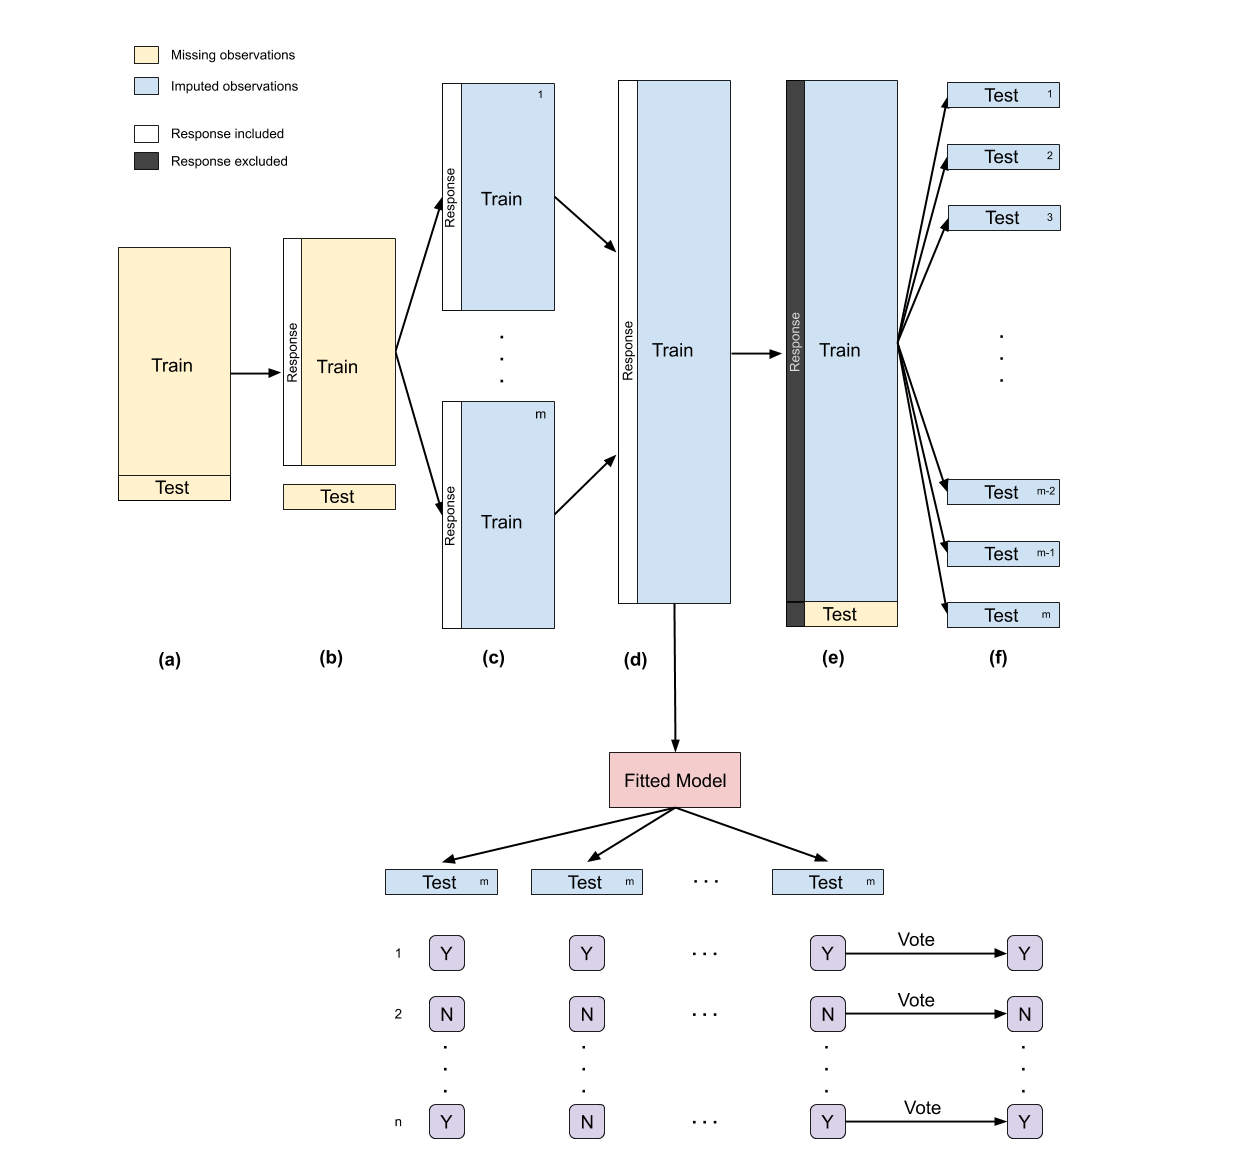
\includegraphics[width=1\linewidth]{images/ensemble-imputation} 

}

\caption{\label{fig:ensemble-imputation}Outline of the algorithm used to pool predictions from multiple imputation.  (a) Step 1. (b) Step 2. (c) Step 3. (d) Step 4.  (e) Step 5.  (f) Step 6.}\label{fig:unnamed-chunk-4}
\end{figure}

The following steps describe the ensemble approach for multiply imputed
data in k-fold cross-validation:

\begin{enumerate}
\def\labelenumi{\arabic{enumi}.}
\tightlist
\item
  Randomly partition the training data into \(k\) folds while retaining
  class proportions
\item
  Define the \(k^{th}\) as the test set and the remaining \(k-1\) folds
  as the training set
\item
  Impute the training set \(m\) times, with the response variable
  \texttt{ECMO\_Survival} included, to create \(m\) imputed training
  sets
\item
  Concatenate the \(m\) imputed training sets into one extended training
  set
\item
  A model is fitted to the extended training set
\item
  The test set is concatenated with the extended training set
\item
  Impute the combined test and extended training set, with the response
  variable \texttt{ECMO\_Survival} excluded, to create \(m\) imputed
  combined test and extended training sets
\item
  Extract the \(m\) test sets
\item
  Make \(m\) predictions on the \(m\) imputed test sets
\item
  Take the majority vote of the \(m\) predictions as the prediction for
  the fitted model
\item
  Validate the prediction against the test set by calculating Cohen's
  Kappa (note there are no missing values for the response variable in
  the data)
\item
  Repeat steps 2-11 \(k\) times and validate the fitted model on each
  training set against the test set for each fold
\item
  Average the \(k\) calculated Cohen's Kappas as the estimated in-sample
  performance
\end{enumerate}

``Rubin's Rules'' \citep{rubin_inference_1976} provide a simple method
for pooling parameters estimates from multiple imputation for linear and
generalized linear models but to the author's knowledge, there has been
insufficient work on estimating the required number of imputations for
estimating posterior probabilities in classification problems. The
classic advice for the choice of \(m\) is between 3 and 5 for moderate
amounts of missing information but it is often beneficial to set \(m\)
higher and create between 20-100 imputations
\citep{van_buuren_flexible_2012}.

The training set is multiply imputed with PMM for \(m=9\) and \(m=99\)
and the predictions pooled by majority vote. There has been sufficient
exploration into pooling of posterior probabilities resulting from
classification problems \textbf{(Citation 1)} \textbf{(Citation 2)}.
\emph{Additionally, not all statistical methods considered produce
posterior probabilities and the comparison of pooled models from
multiple imputation is an area ripe for more analysis.} Indeed, others
have pooled predictions from various machine learning methods by taking
the majority vote \textbf{(Zavrakidis)} \textbf{(Citation 2)}, and
comparing prediction performance. The combination can be implemented
using a variety of strategies, among which majority vote is one of the
simplest, and has been found to be just as effective as more complicated
schemes \citep{lam_optimal_1995}.

\subsection{Feature Selection}\label{feature-selection}

One of the goals of this analysis is to identify the variables most
useful for accurate prediction. There are various methods that can be
used for feature selection: stepwise selection, Recursive Feature
Elimination (RFE), LASSO regularization, and Principal Component
Analysis (PCA). However, some of these methods are either highly
criticized, dependent on the classification method considered, or cannot
be integrated into the ensemble cross-validation approach used. Stepwise
selection, while very common, is only applicable to regression models
and it is often criticised \citep{kemp_applied_2003}; problems include
falsely narrow confidence intervals for effects and predicted values
\citep{altman_bootstrap_1989} and multiple hypothesis testing inflating
risks of capitalising on chance features of the data
\citep{altman_practical_1991}, such as noise covariates gaining entry
into the model when the number of candidate variables is large
\citep{derksen_backward_1992}. RFE is an iterative procedure analogous
of backward feature selection. A new classifier is trained on a subset
of the features and the importance of the feature is a measure of the
change in performance. The training time scales linearly with the number
of classifiers to be trained \citep{guyon_gene_2002}. Both logistic
regression with LASSO regularization \citep{tibshirani_regression_1996}
and the analogous Sparse Discriminant Analysis
\citep{clemmensen_sparse_2011} are embedded feature selection methods
that are dependent on the classification method.

Principal Component Analysis (PCA) \citep{f.r.s_liii._1901} is a feature
extraction method that is independent of the classification method. The
training set are orthogonally transformed into new uncorrelated
variables called principal components that are linear combinations of
the original variables. Feature extraction is accomplished by selecting
the \(k\) largest principal components that contain a chosen percent of
the variance in the original feature space.

PCA can also be used for feature selection by calculating the
contribution of each variable to the extracted features
\citep{song_feature_2010}. Let \(C_i\) be the contribution of a given
variable on the principal component, \(\text{V}_i\), and let
\(\lambda_i\) be the eigenvalue of \(\text{V}_i\), where
\(\text{V}_{i} = \lambda_i \text{C}_i\). Eigenvalues measure the amount
of variation retained by each principal component. The total
contribution of a variable, \(\text{C}_j\), on explaining the variations
retained by \(k\) extracted features, \(\text{V}_1, ..., \text{V}_k\),
is

\[
\text{C}_j = \sum^k_{i=1}\lambda_{ij} \text{C}_{ij} = \sum^k_{p=1} \vert \text{V}_{ij} \vert 
\]

The \(\text{C}_j\) are sorted in descending order where \(\text{C}_1\)
contributes the most variation to the extracted principal components
among all the \(\text{C}_j\) for \(j=1,2,...p\), variables.

\newpage

\section{Results}\label{results}

\subsection{Missing Data Patterns}\label{missing-data-patterns}

Before imputation, and indeed multiple imputation, it is important to
inspect the missingness patterns in the data and check assumptions.
Figure \ref{fig:missing-data} shows the missingness patterns in the
dataset, where a black bar represents a missing value. Table
\ref{tab:missing-statistics} provides some measures about variable
dependence in the dataset. The first row shows the probability of
observed values for each variable. The following are coefficients that
give insight into how the variables are connected in terms of
missingness. \(\mathbf{Influx}\) is the ratio of the number of variables
pairs \((Y_j, ~Y_k)\) with \(Y_j\) missing and \(Y_k\) observed, divided
by the total number of observed data. For a variable that is entirely
missing, influx is 1, and 0 for if the variable is complete.
\(\mathbf{Outflux}\) is defined in the opposit manner, by dividing the
number of pairs \((Y_j, ~Y_k)\) with \(Y_j\) observed and \(Y_k\)
missing, by the total number of complete cells. For a completely
observed variable, outflux will have a value of 1 and 0 if completely
missing. Outflux gives an indication of how useful the variable will be
for imputing other variables in the dataset, while influx is an
indicator for how easily the variable can be imputed. Table
\ref{tab:missing-patterns} shows that all variables will be useful
during impuation except \texttt{PreECMO\_Albumin}. A high outflux
variable might turn out to be useless for the imputation procedure if it
is unrelated to the incomplete variables, while the usefulness of a
highly predictive variables is severely limited by a low outflux value
(Van Buuren 2012). \textbf{Mention \ref{fig:missing-data})}

\begin{figure}[H]

{\centering 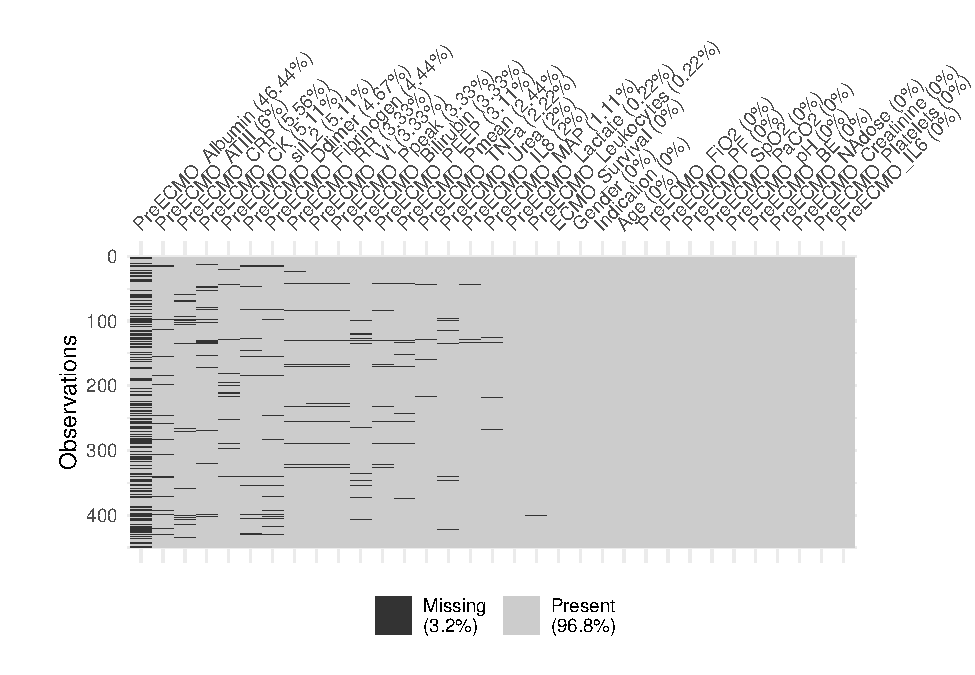
\includegraphics[width=1\linewidth]{figure/graphics-missing-data-1} 

}

\caption{\label{fig:missing-data}Visual representation of missing observations in the ARDS dataset.}\label{fig:missing-data}
\end{figure}

\begin{itemize}
\tightlist
\item
  It can be difficult or impossible to determine if the data are MCAR.
  Figure \ref{fig:missing-data} shows that many missing values occur in
  observations with other missing values. Missing values could be
  conditionally dependent on other variables, in which case the data
  would be MAR. The missing values could also be due to some unknown
  mechanism at the time of recording (\emph{i.e.} a failure of the
  measurement device) that happens to effect multiple readings (the
  biomarkers are measured from blood samples and measurements are likely
  done in batches). In this case the data would be MCAR. Without more
  information, this analysis assumes the data is MCAR.
\end{itemize}

\subsection{Prediction Performance}\label{prediction-performance}

The experimentation phase of this study involved three methods for
handling missing data: (a) complete case analysis with the variable
\texttt{PreECMO\_Albumin} dropped from the analysis due to 46.44\%
missingness, (b) mean imputation on variables with missing values, (c)
imputation via the MICE algorithm implemented with PMM.

\begin{table}[!h]

\caption{\label{tab:unnamed-chunk-5}\label{tab:cv-kappa} Averaged Cohen's Kappa for each model fitted in cross-validation.  The tuned parameters for K-Nearest Neighbors and Random Forests are (a) K=5 and mtry=13 (b) K=13 and mtry=15, respectively.}
\centering
\fontsize{10}{12}\selectfont
\begin{tabular}{lrrrrr}
\toprule
  & Logit & LDA & QDA & KNN & RF\\
\midrule
Complete Case & 0.139 & 0.205 & 0.038 & 0.053 & 0.035\\
Mean & 0.191 & 0.220 & 0.040 & 0.136 & 0.085\\
PMM9 & 0.179 & 0.124 & 0.106 & 0.088 & 0.136\\
PMM99 & 0.185 & 0.158 & 0.037 & 0.127 & 0.177\\
\bottomrule
\end{tabular}
\end{table}

Table \ref{tab:cv-kappa} shows the averaged Kappa from each analysis in
10-fold cross-validation. In complete case analysis and mean imputaion,
LDA is the highest performer. While for predictive mean-matching with
\(m=9\) and \(m=99\) logistic regression has the highest averaged Kappa.

\subsubsection{Validation on Test Set}\label{validation-on-test-set}

Using the parameters values learned from 10-fold cross-validation in
Table \ref{tab:cv-kappa}, models were fit to the full training set and
validated against the test set. Trained parameters for K-nearest
neighbors and random forests on \(m=9\) imputed datasets were \(K=5\)
and \(mtry=13\), respectively, and on \(m=99\) imputed datasets were
\(K=13\) and \(mtry=15\), respectively.

\begin{table}[!h]

\caption{\label{tab:unnamed-chunk-6}\label{tab:metrics} Pooled performance results of trained models validated on test set.}
\centering
\fontsize{10}{12}\selectfont
\begin{tabular}{lccccc}
\toprule
 &  & Sensitivity & Specificity & Accuracy & Kappa\\
\midrule
 & Logit & 0.200 & 0.814 & 0.658 & 0.015\\

 & LDA & 0.200 & 0.847 & 0.684 & 0.054\\

 & QDA & 0.000 & 0.966 & 0.722 & -0.048\\

 & KNN & 0.300 & 0.847 & 0.709 & 0.161\\

\multirow{-5}{*}{\raggedright\arraybackslash Complete Case} & RF & 0.050 & 0.966 & 0.734 & 0.022\\
\cmidrule{1-6}
 & Logit & 0.222 & 0.894 & 0.732 & 0.137\\

 & LDA & 0.148 & 0.894 & 0.714 & 0.051\\

 & QDA & 0.111 & 0.882 & 0.696 & -0.008\\

 & KNN & 0.222 & 0.824 & 0.679 & 0.050\\

\multirow{-5}{*}{\raggedright\arraybackslash Mean} & RF & 0.185 & 0.965 & 0.777 & 0.197\\
\cmidrule{1-6}
 & Logit & 0.222 & 0.906 & 0.741 & 0.153\\

 & LDA & 0.148 & 0.906 & 0.723 & 0.067\\

 & QDA & 0.111 & 0.882 & 0.696 & -0.008\\

 & KNN & 0.222 & 0.847 & 0.696 & 0.077\\

\multirow{-5}{*}{\raggedright\arraybackslash PMM (m=9)} & RF & 0.148 & 0.941 & 0.750 & 0.116\\
\cmidrule{1-6}
 & Logit & 0.333 & 0.906 & 0.768 & 0.274\\

 & LDA & 0.185 & 0.906 & 0.732 & 0.111\\

 & QDA & 0.111 & 0.894 & 0.705 & 0.006\\

 & KNN & 0.185 & 0.882 & 0.714 & 0.080\\

\multirow{-5}{*}{\raggedright\arraybackslash PMM (m=99)} & RF & 0.185 & 0.929 & 0.750 & 0.144\\
\bottomrule
\end{tabular}
\end{table}

\subsection{Feature Selection}\label{feature-selection-1}

The number of principal components retained is based on the proportion
of variance. At least 16 principal components are needed to explain 80\%
of the variance in the imputed training data and at least 15 principal
components for the complete case analysis. The red dashed lines in
Figure \ref{fig:feature-importance-pca} indicate the expected average
contribution. If the contribution of the variables were uniform, the
expected value would be \(\frac{1}{\text{no. of variables}} =\) 0.03.
For a given component, an observation with a contribution larger than
this cutoff could be considered as important in contributing to the
component.

\begin{figure}[H]

{\centering 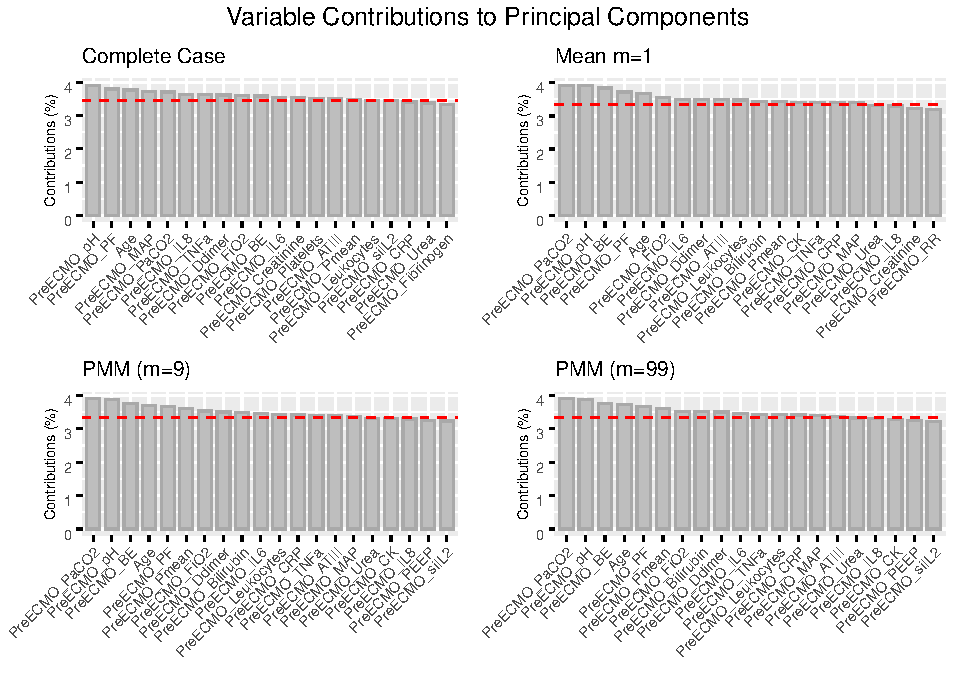
\includegraphics[width=1\linewidth]{figure/graphics-unnamed-chunk-7-1} 

}

\caption{\label{fig:feature-importance-pca}Contribution of variables to the principal components whose cumulative sum explains >80\% of the variation in the data.}\label{fig:unnamed-chunk-7}
\end{figure}

\newpage

\section{Discussion}\label{discussion}

\subsection{Model Performance}\label{model-performance}

\textbf{Logistic Regression}\\
For complete-case analysis, mean imputation, and predictive
mean-matching, logistic regression does not meet the ``one in ten
rule'', a rule of thumb stating that a logistic regression models give
stable estimates for the covariates if there are at least 10
observations of the least frequent class per covariate.

\textbf{LDA}\\
Can perform better than logistic regression when the covariates are
normally distributed \textbf{(CITATION)}, which they are in this case
after Yeo-Johnson transformation.

\textbf{QDA}

\textbf{K-Nearest Neighbors}

\textbf{Random Forests Fails}

\begin{itemize}
\item
  Sparsity - When the data are very sparse, it's very plausible that for
  some node, the bootstrapped sample and the random subset of features
  will collaborate to produce an invariant feature space. There's no
  productive split to be had, so it's unlikely that the children of this
  node will be at all helpful.
\item
  One surprising consequence is that trees that work well for
  nearest-neighbor search problems can be bad candidates for forests
  without sufficient subsampling, due toa lack of diversity.
  \textbf{(Tang et al. 2018)}
\item
  Data are not axis-aligned - Suppose that there is a diagonal decision
  boundary in the space of two features, \(x_1\) or \(x_2\). Even if
  this is the only relevant dimension to your data, it will take an
  ordinary random forest model many splits to describes that diagonal
  boundary. This is because each split is oriented perpendicular to the
  axis of either \(x_1\) or \(x_2\).
\item
  XGBoost, Rotation forest (PCA rotation) may do better
\end{itemize}

\subsection{Important Features for
Prediction}\label{important-features-for-prediction}

\begin{itemize}
\tightlist
\item
  Mention poor model performance
\item
  Correlation heatmap
\item
  Results from PCA
\item
  \textbf{Refer to Figure \ref{fig:feature-importance-pca} in Appendix A
  for feature importance plots from PCA analysis}
\end{itemize}

\subsection{Conclusion}\label{conclusion}

\begin{itemize}
\tightlist
\item
  Summary of proceedure
\item
  Summary of results
\item
  Possible improvements and future work
\end{itemize}

\subsubsection{Feature Selection}\label{feature-selection-2}

\begin{itemize}
\tightlist
\item
  Model dependent methods for feature extraction may
\end{itemize}

\newpage

\section{Appendices}\label{appendices}

\subsection{A. Additional Exploratory Data
Analysis}\label{a.-additional-exploratory-data-analysis}

\begin{figure}[H]

{\centering 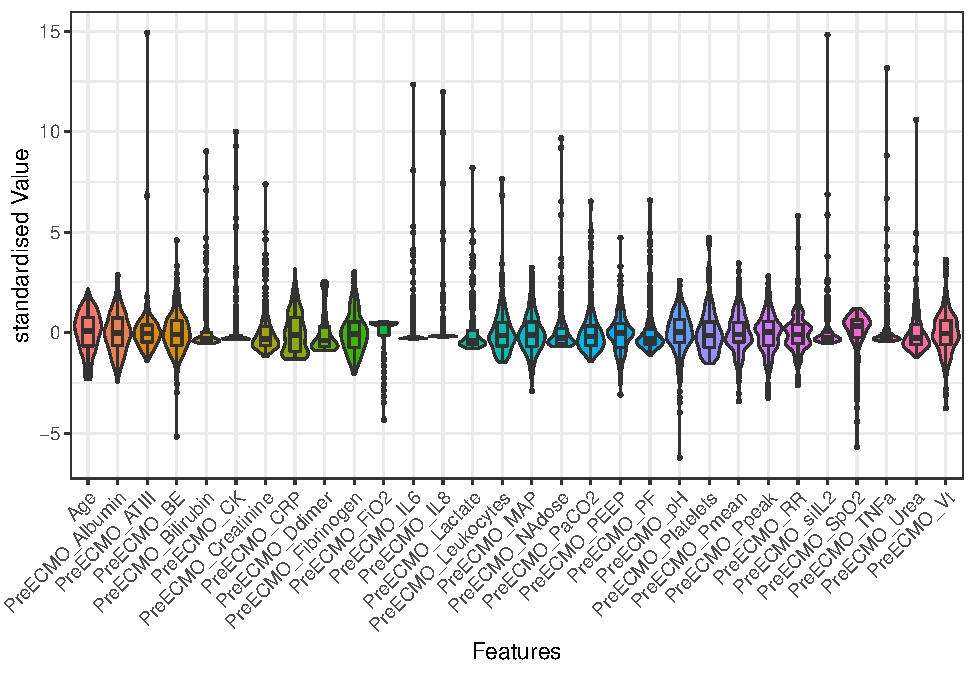
\includegraphics[width=1\linewidth]{figure/graphics-unnamed-chunk-8-1} 

}

\caption{\label{fig:heatmap-standardized}Heatmap of standardized and transformed variables.}\label{fig:unnamed-chunk-8}
\end{figure}

\subsection{B. Algorithms}\label{b.-algorithms}

\subsubsection{Random Forests Algorithm}\label{random-forests-algorithm}

The random forests algorithm depicted is adapted from
\citep{hastie_elements_2009}.

\begin{algorithm}[H]

\caption{Random Forest Classifier}
\DontPrintSemicolon
\SetAlgoLined
\BlankLine

\begin{enumerate}
  \item For ($b=1$ to B):
    \begin{enumerate}
      \item Draw a bootstrap sample $\mathbf{Z*}$ of the size $N$ from the training data.
      \item Grow a random-forest tree $T_b$ to the bootstrapped data, by recursively repreating the following steps for each terminal node of the tree, until the minimum node size $n_{min}$ is reached.
      \begin{enumerate}
        \item Select $mtry$ variables at random from the $p$ covariates. 
        \item Pick the best covariate/split-point among the $mtry$. 
        \item Split the node into two daughter nodes. 
      \end{enumerate}
    \end{enumerate}
  \item Output the ensemble of trees $\{T_B\}^B_1$
\end{enumerate}
\BlankLine

Let $\hat{Y}_b(x)$ be the class prediction of the $b^{\text{th}}$ random-forest tree.  Then a new observation, $x$, is classified as:

$$\hat{Y}^B_{\text{rf}}(x) = \text{majority vote } \left\{ \hat{Y}_b(x) \right\}^B_1$$

\end{algorithm}

\subsubsection{MICE Algorithm}\label{mice-algorithm}

The MICE algorithm is adapted from \citep{van_buuren_flexible_2012}.

\begin{algorithm}[H]

\caption{Multiple Imputation via Chained Equations}
\DontPrintSemicolon
\SetAlgoLined
\BlankLine

\begin{enumerate}
  \item Specify an imputation model $P(Y^{\text{mis}}_j \vert Y^{\text{obs}}_j, Y_{-j}, R)$ for variable $Y_j$ with $j=1,...,p$
  \item For each $j$, fill in starting imputation $Y^0_j$ by random draws from $Y^{\text{obs}}_j$
  \item Repeat for $t=1,...,T:$
  \item Repeat for $j=1,...,p:$
  \item Define $Y^t_{-j} = (Y^t_1,...,T^t_{j-1}, Y^{t-1}_{j+1},..., Y^{t-1}_p)$ as the currently complete data except $Y_j$ 
  \item Draw $\phi^t_j \sim P(\phi^t_j \vert Y^{\text{obs}}_j, Y^t_{-j}, R)$.
  \item Draw imputations from $Y^t_j \sim P(Y^{ \text{mis} }_j \vert Y^{ \text{obs} }_j, Y^t_{-j}, R, \phi^t_j)$.
  \item End repeat $j$.
  \item End repeat $t$.

\end{enumerate}
\BlankLine

\end{algorithm}

\subsubsection{Majority Vote}\label{majority-vote}

\textbf{(Alexandre et al. 2001)} There has been some interest on the
comparative performance of the sum and product rules (or the arithmetic
and geometric means) (Kittler et al., 1996; Tax et al., 1997; Kittler et
al., 1998). The arithmetic mean is one of the most frequently used
combination rules since it is easy to implement and normally produces
good results.

In (Kittler et al., 1998), the authors show that for combination rules
based on the sum, such as the arithmetic mean, and for the case of
classifiers working in different feature spaces, the arithmetic mean is
less sensitive to errors than geometric mean.

In fact (Alexandre et al. 2001) show that for classification problems
with two classes, that give estimates of the a posteriori probabilities
that sum to one the combination rules arithmetic mean (or the sum) and
the geometric mean (or the product) are equivalent.

\subsection{C. Additional Missing Data
Diagnostics}\label{c.-additional-missing-data-diagnostics}

\begin{figure}[H]

{\centering \includegraphics[width=1\linewidth]{figure/graphics-unnamed-chunk-10-1} 

}

\caption{\label{fig:missing-data-patterns1}Missing data patterns.  Each row corresponds to a missing data pattern (1=observed, 0=missing).  Rows and columns are sorted in increasing amounts of missing information.  The last column and row contain row and column counts, respectively.}\label{fig:unnamed-chunk-10}
\end{figure}

\begin{figure}[H]

{\centering 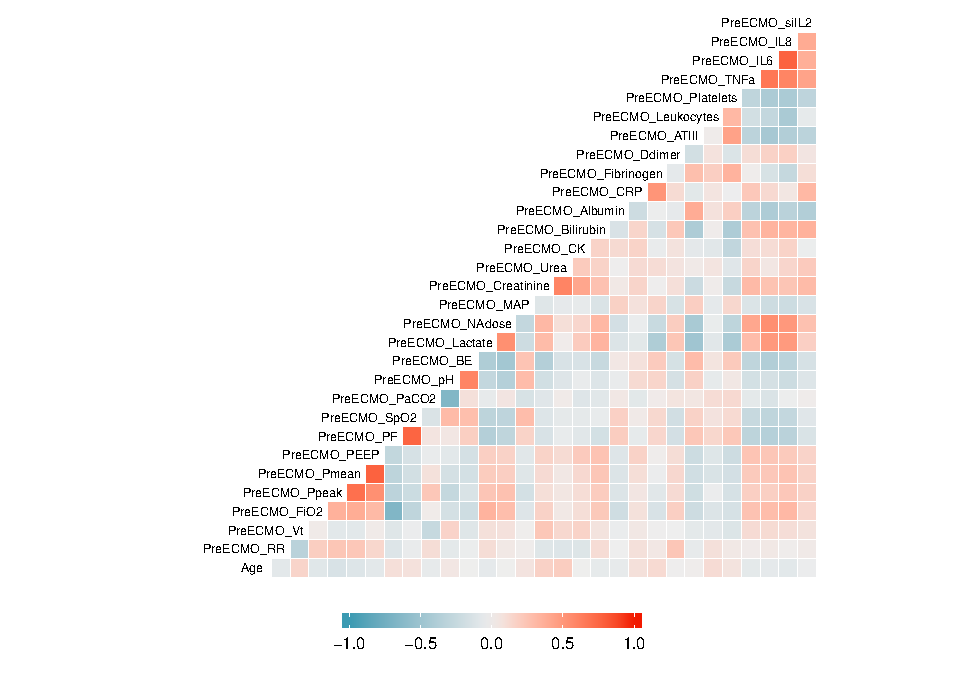
\includegraphics[width=1\linewidth]{figure/graphics-unnamed-chunk-11-1} 

}

\caption{\label{fig:missing-data-patterns2}Missing data patterns.  Each row corresponds to a missing data pattern (1=observed, 0=missing).  Rows and columns are sorted in increasing amounts of missing information.  The last column and row contain row and column counts, respectively.}\label{fig:unnamed-chunk-11}
\end{figure}

\begin{verbatim}

 Variables sorted by number of missings: 
           Variable       Count
    PreECMO_Albumin 0.464444444
      PreECMO_ATIII 0.060000000
        PreECMO_CRP 0.055555556
         PreECMO_CK 0.051111111
      PreECMO_siIL2 0.051111111
     PreECMO_Ddimer 0.046666667
 PreECMO_Fibrinogen 0.044444444
         PreECMO_RR 0.033333333
         PreECMO_Vt 0.033333333
      PreECMO_Ppeak 0.033333333
  PreECMO_Bilirubin 0.033333333
       PreECMO_PEEP 0.031111111
      PreECMO_Pmean 0.024444444
       PreECMO_TNFa 0.022222222
       PreECMO_Urea 0.020000000
        PreECMO_IL8 0.020000000
        PreECMO_MAP 0.011111111
    PreECMO_Lactate 0.002222222
 PreECMO_Leukocytes 0.002222222
      ECMO_Survival 0.000000000
             Gender 0.000000000
         Indication 0.000000000
                Age 0.000000000
       PreECMO_FiO2 0.000000000
         PreECMO_PF 0.000000000
       PreECMO_SpO2 0.000000000
      PreECMO_PaCO2 0.000000000
         PreECMO_pH 0.000000000
         PreECMO_BE 0.000000000
     PreECMO_NAdose 0.000000000
 PreECMO_Creatinine 0.000000000
  PreECMO_Platelets 0.000000000
        PreECMO_IL6 0.000000000
\end{verbatim}

\subsubsection{Visual Insepction of
Imputations}\label{visual-insepction-of-imputations}

\begin{table}[!h]

\caption{\label{tab:unnamed-chunk-12}\label{tab:missing-statistics} Missing pattern statistics for variables in dataset.}
\centering
\fontsize{10}{12}\selectfont
\begin{tabular}{lrrr}
\toprule
  & Proportion & Influx & Outflux\\
\midrule
ECMO\_Survival & 1.00 & 0.00 & 1.00\\
Gender & 1.00 & 0.00 & 1.00\\
Indication & 1.00 & 0.00 & 1.00\\
Age & 1.00 & 0.00 & 1.00\\
PreECMO\_RR & 0.97 & 0.03 & 0.85\\
\addlinespace
PreECMO\_Vt & 0.97 & 0.03 & 0.85\\
PreECMO\_FiO2 & 1.00 & 0.00 & 1.00\\
PreECMO\_Ppeak & 0.97 & 0.03 & 0.85\\
PreECMO\_Pmean & 0.98 & 0.02 & 0.90\\
PreECMO\_PEEP & 0.97 & 0.03 & 0.85\\
\addlinespace
PreECMO\_PF & 1.00 & 0.00 & 1.00\\
PreECMO\_SpO2 & 1.00 & 0.00 & 1.00\\
PreECMO\_PaCO2 & 1.00 & 0.00 & 1.00\\
PreECMO\_pH & 1.00 & 0.00 & 1.00\\
PreECMO\_BE & 1.00 & 0.00 & 1.00\\
\addlinespace
PreECMO\_Lactate & 1.00 & 0.00 & 0.99\\
PreECMO\_NAdose & 1.00 & 0.00 & 1.00\\
PreECMO\_MAP & 0.99 & 0.01 & 0.97\\
PreECMO\_Creatinine & 1.00 & 0.00 & 1.00\\
PreECMO\_Urea & 0.98 & 0.02 & 0.94\\
\addlinespace
PreECMO\_CK & 0.95 & 0.05 & 0.87\\
PreECMO\_Bilirubin & 0.97 & 0.03 & 0.91\\
\textbf{PreECMO\_Albumin} & \textbf{0.54} & \textbf{0.46} & \textbf{0.26}\\
PreECMO\_CRP & 0.94 & 0.05 & 0.88\\
PreECMO\_Fibrinogen & 0.96 & 0.04 & 0.85\\
\addlinespace
PreECMO\_Ddimer & 0.95 & 0.04 & 0.86\\
PreECMO\_ATIII & 0.94 & 0.06 & 0.84\\
PreECMO\_Leukocytes & 1.00 & 0.00 & 0.99\\
PreECMO\_Platelets & 1.00 & 0.00 & 1.00\\
PreECMO\_TNFa & 0.98 & 0.02 & 0.93\\
\addlinespace
PreECMO\_IL6 & 1.00 & 0.00 & 1.00\\
PreECMO\_IL8 & 0.98 & 0.02 & 0.93\\
PreECMO\_siIL2 & 0.95 & 0.05 & 0.87\\
\bottomrule
\end{tabular}
\end{table}

\begin{figure}[H]

{\centering 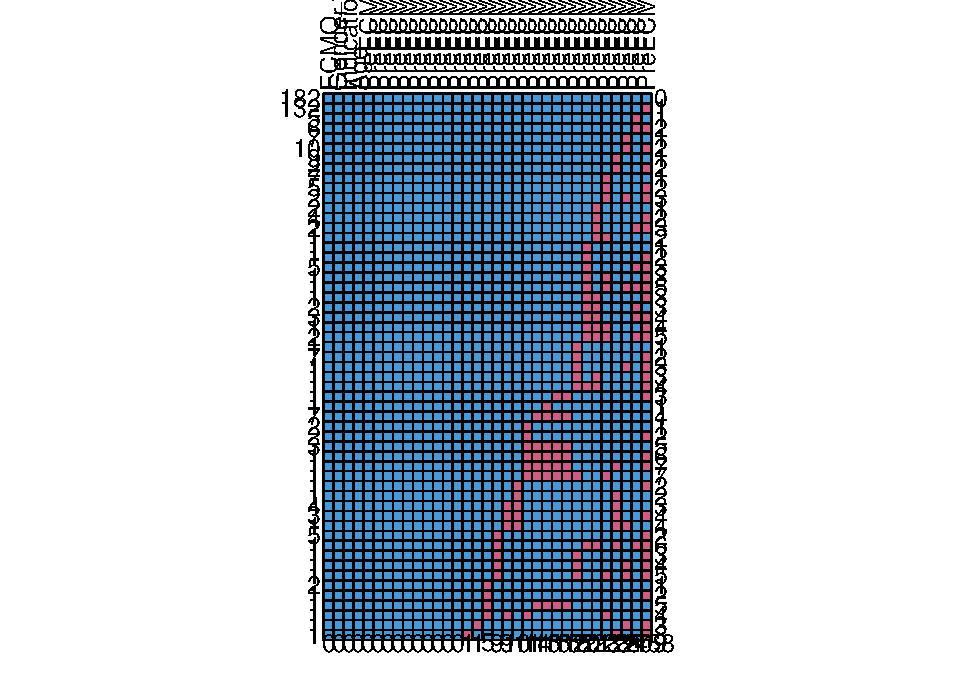
\includegraphics[width=1\linewidth]{figure/graphics-unnamed-chunk-13-1} 

}

\caption{\label{fig:xyplot-mean}Scatterplot of each imputed dataset}\label{fig:unnamed-chunk-13}
\end{figure}

\begin{figure}[H]

{\centering 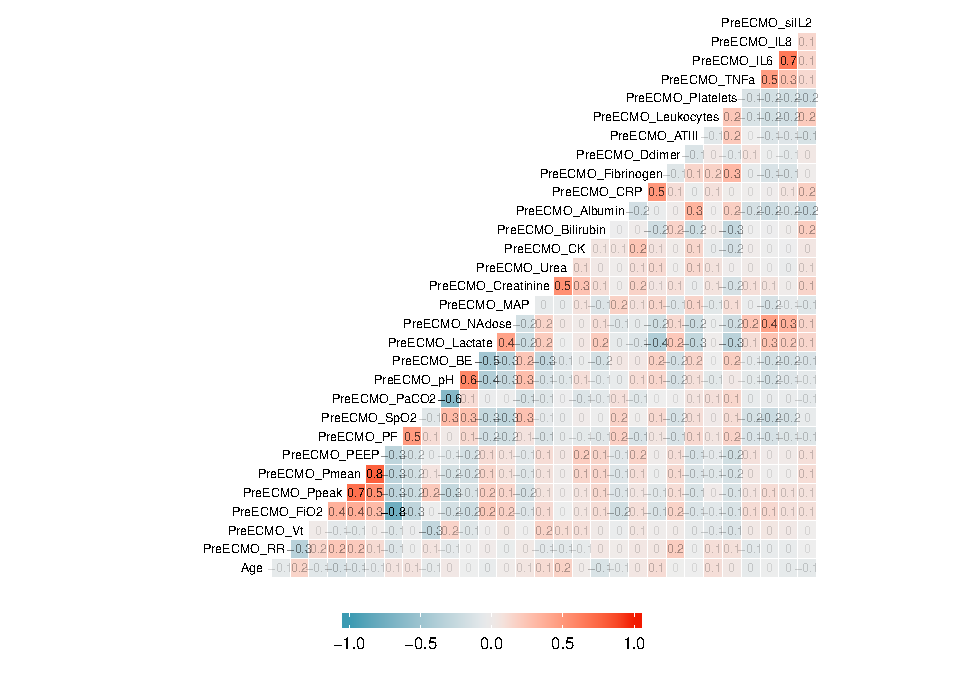
\includegraphics[width=1\linewidth]{figure/graphics-unnamed-chunk-14-1} 

}

\caption{\label{fig:xyplot-pmm}Scatterplot of each imputed dataset}\label{fig:unnamed-chunk-14}
\end{figure}

\begin{itemize}
\item
  \textbf{xyplot checking distributions of original and imputed data for
  MEAN imputation}
\item
  \textbf{xyplot checking distributions of original and imputed data for
  PMM imputation}
\item
  \textbf{density plot of original and imputed data for MEAN imputation}
\item
  \textbf{density plot of original and imputed data for PMM imputation}
\end{itemize}

This plot compares the density of observed data with the ones of imputed
data. We expect them to be similar (though not identical) under MAR
assumption.

\subsubsection{Convergence Monitoring}\label{convergence-monitoring}

\begin{itemize}
\tightlist
\item
  \textbf{Plot of convergence}
\end{itemize}

\subsection{D. Feature Selection}\label{d.-feature-selection}

\begin{figure}[H]

{\centering 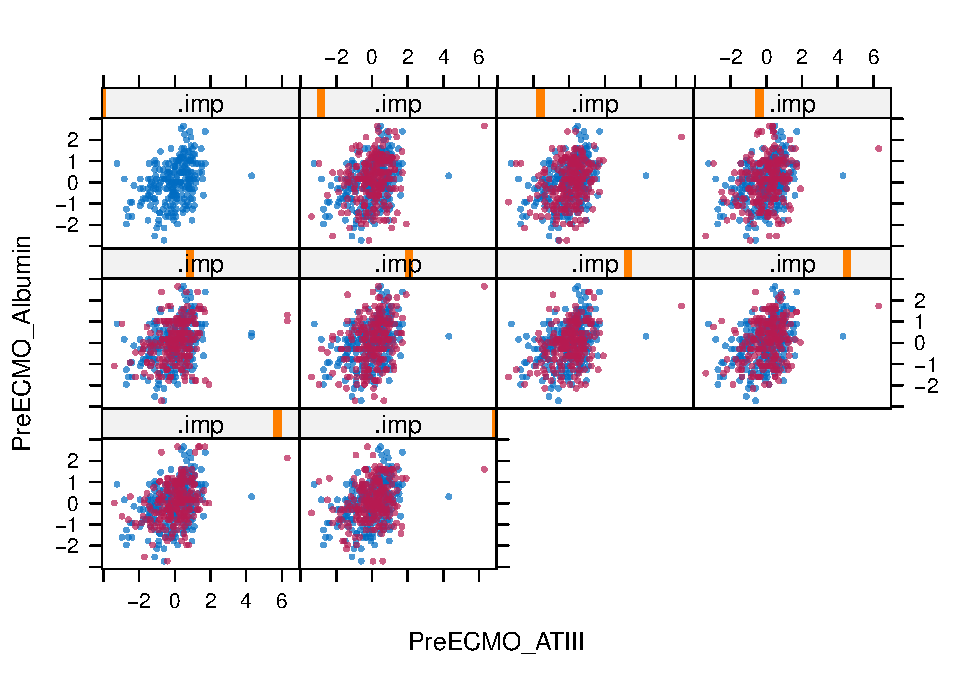
\includegraphics[width=1\linewidth]{figure/graphics-unnamed-chunk-15-1} 

}

\caption{\label{fig:rfe-logit}Ordered feature importance from Logit model}\label{fig:unnamed-chunk-15}
\end{figure}

\subsection{E. Code Structure}\label{e.-code-structure}

The code organization is described in Figure \ref{fig:r-code-chart}.
\texttt{libraries.R} contains all the libraries used in the analysis.
\texttt{functions.R} contains functions used in \texttt{training.R} and
\texttt{model-evaluation.R}. The ensemble cross-validation algorithm is
done in the \texttt{crossValidation()} function. The data is initially
cleaned and split into test and training sets in \texttt{preprocess.R}.
The cleaned datasets are saved to \texttt{processed-data.RData} for use
in \texttt{training.R} and in creating tables and figures in the thesis
rmarkdown. The training data is loaded into \texttt{training.R} where
each of the five classification methods are trained via ensemble
cross-validation. This is done for the four imputation methods: complete
case analysis, mean imputation, MICE using PMM for \(m=9\), and MICE
using PMM for \(m=99\) imputed datasets. The trained models for each
imputation method are saved into separate \texttt{trained-models.RData}.
The methods are then then fit to the full training set in
\texttt{model-evaluation.R} using the trained parameters found in
\texttt{training.R}. The final fitted models are evaluated on the test
set and the fitted models and performance metrics are saved to
\texttt{metrics.RData}.

\begin{figure}[H]

{\centering 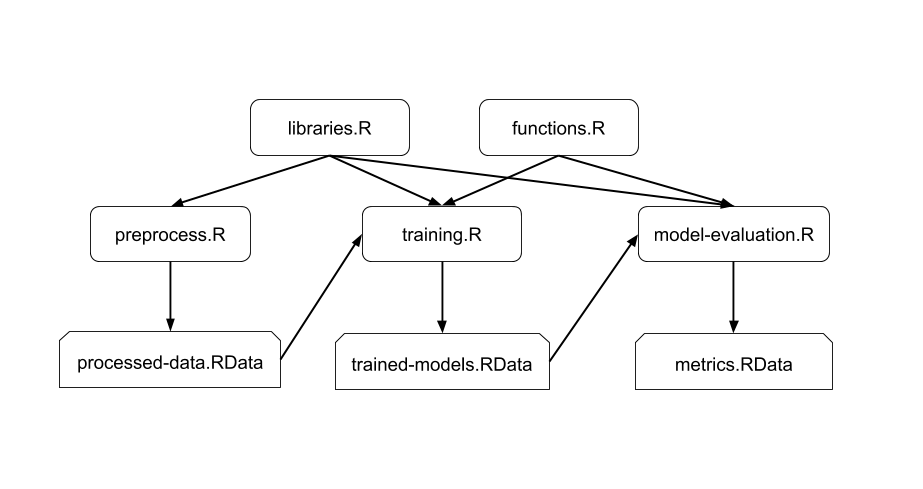
\includegraphics[width=1\linewidth]{images/r-code-chart} 

}

\caption{\label{fig:r-code-chart}Flowchart of code structure.}\label{fig:unnamed-chunk-16}
\end{figure}

\subsection{F. OLD PLOTS \& FIGURES}\label{f.-old-plots-figures}

\begin{table}[!h]

\caption{\label{tab:unnamed-chunk-20}\label{tab:cc-metrics} Complete case analysis accuracy metrics.  The tuned hyperparameters for K-Nearest Neighbors and Random Forests are K=5 and mtry=11, respectively.}
\centering
\fontsize{10}{12}\selectfont
\begin{tabular}{lrrrr}
\toprule
  & Sensitivity & Specificity & Accuracy & Kappa\\
\midrule
Logit & 0.20 & 0.814 & 0.658 & 0.015\\
LDA & 0.20 & 0.847 & 0.684 & 0.054\\
QDA & 0.00 & 0.966 & 0.722 & -0.048\\
\textbf{KNN} & \textbf{0.30} & \textbf{0.847} & \textbf{0.709} & \textbf{0.161}\\
RF & 0.05 & 0.966 & 0.734 & 0.022\\
\bottomrule
\end{tabular}
\end{table}

\begin{table}[!h]

\caption{\label{tab:unnamed-chunk-21}\label{tab:mean-metrics} Mean imputation accuracy metrics (m=1).  The tuned hyperparameters for K-Nearest Neighbors and Random Forests are K=5 and mtry=11, respectively.}
\centering
\fontsize{10}{12}\selectfont
\begin{tabular}{lrrrr}
\toprule
  & Sensitivity & Specificity & Accuracy & Kappa\\
\midrule
Logit & 0.222 & 0.894 & 0.732 & 0.137\\
LDA & 0.148 & 0.894 & 0.714 & 0.051\\
QDA & 0.111 & 0.882 & 0.696 & -0.008\\
KNN & 0.222 & 0.824 & 0.679 & 0.050\\
\textbf{RF} & \textbf{0.185} & \textbf{0.965} & \textbf{0.777} & \textbf{0.197}\\
\bottomrule
\end{tabular}
\end{table}

\begin{table}[!h]

\caption{\label{tab:unnamed-chunk-22}\label{tab:pmm-metrics} MICE via predictive mean matching accuracy metrics (m=9).  The tuned hyperparameters for K-Nearest Neighbors and Random Forests are K=5 and mtry=13, respectively.}
\centering
\fontsize{10}{12}\selectfont
\begin{tabular}{lrrrr}
\toprule
  & Sensitivity & Specificity & Accuracy & Kappa\\
\midrule
\textbf{Logit} & \textbf{0.222} & \textbf{0.906} & \textbf{0.741} & \textbf{0.153}\\
LDA & 0.148 & 0.906 & 0.723 & 0.067\\
QDA & 0.111 & 0.882 & 0.696 & -0.008\\
KNN & 0.222 & 0.847 & 0.696 & 0.077\\
RF & 0.148 & 0.941 & 0.750 & 0.116\\
\bottomrule
\end{tabular}
\end{table}

\begin{table}[!h]

\caption{\label{tab:unnamed-chunk-23}\label{tab:pmm99-metrics} MICE via predictive mean matching accuracy metrics (m=99).  The tuned hyperparameters for K-Nearest Neighbors and Random Forests are K=13 and mtry=15, respectively.}
\centering
\fontsize{10}{12}\selectfont
\begin{tabular}{lrrrr}
\toprule
  & Sensitivity & Specificity & Accuracy & Kappa\\
\midrule
\textbf{Logit} & \textbf{0.333} & \textbf{0.906} & \textbf{0.768} & \textbf{0.274}\\
LDA & 0.185 & 0.906 & 0.732 & 0.111\\
QDA & 0.111 & 0.894 & 0.705 & 0.006\\
KNN & 0.185 & 0.882 & 0.714 & 0.080\\
RF & 0.185 & 0.929 & 0.750 & 0.144\\
\bottomrule
\end{tabular}
\end{table}

\newpage

\bibliography{bibliography.bib}


\end{document}
